\documentclass[letterpaper]{article}
\usepackage[spanish]{babel}
\usepackage[right=2.2cm,left=2.2cm]{geometry}
\usepackage{graphicx}
\usepackage{float}
\usepackage{hyperref}
\usepackage{grffile}
\usepackage{longtable}
\usepackage{wrapfig}
\usepackage{rotating}

\usepackage[normalem]{ulem}
\usepackage{amsmath}
\usepackage{textcomp}
\usepackage{amssymb}
\usepackage{capt-of}
\usepackage{fancyhdr}
\usepackage{subfiles}

\hypersetup{
  pdfkeywords={},
  pdfsubject={},
  pdflang={Spanish}
}
\usepackage{minted}
\usepackage{xcolor}

\definecolor{LightGray}{gray}{0.9}
%\definecolor{DarkGray}{gray}{0.1}

%\pagecolor{DarkGray}

\usemintedstyle{emacs}

\renewcommand{\listingscaption}{Código}

\graphicspath{{./img/}}
\pagestyle{fancy}
\fancyfoot[R]{\thepage}
\fancyfoot[C]{
\includegraphics[width=0.1\textwidth]{inge_logo}}
\fancyhead[L]{\leftmark}
\fancyhead[R]{\rightmark}

\begin{document}
\begin{titlepage}
  \centering{
    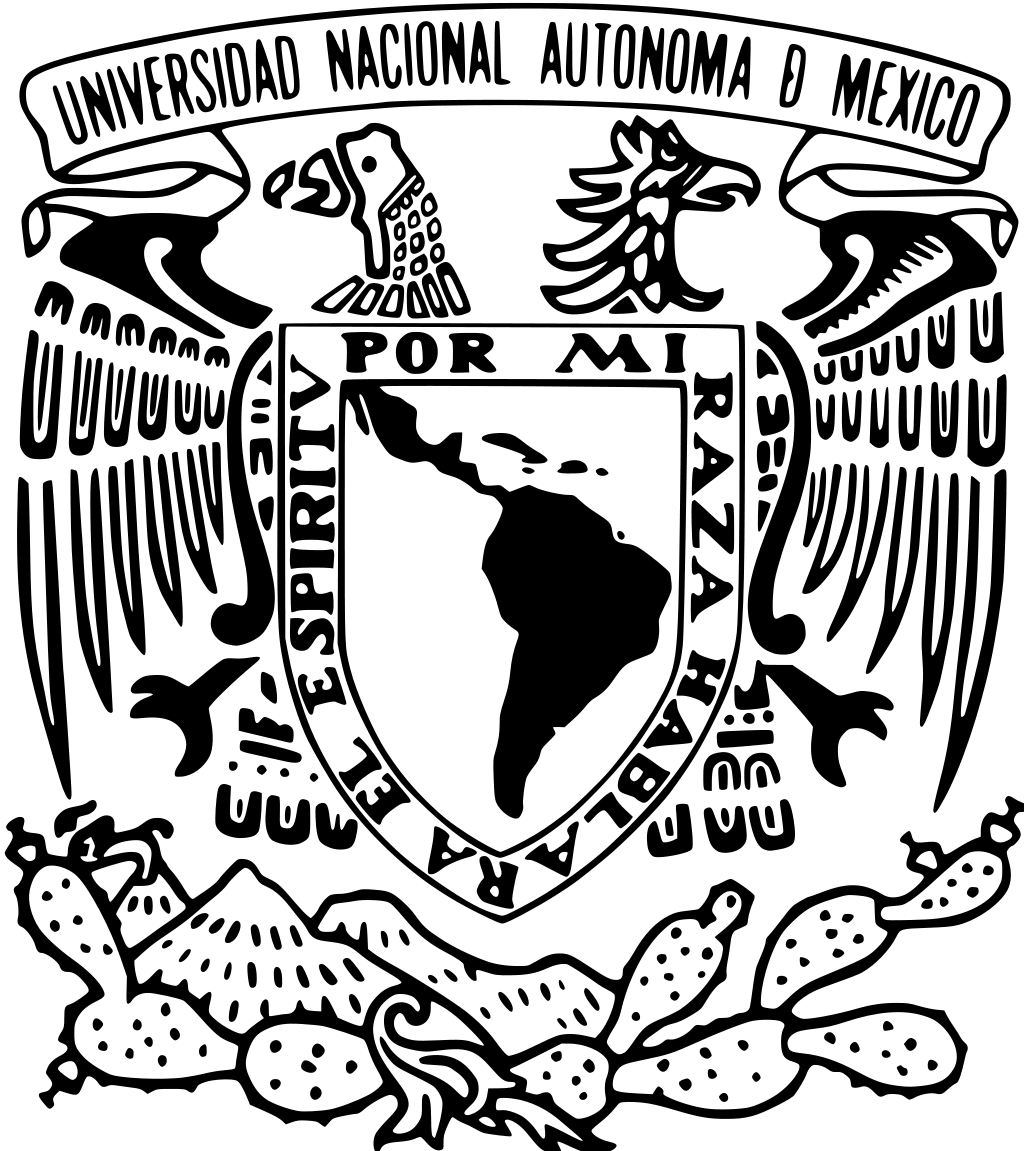
\includegraphics[width=0.3\textwidth]{unam_logo}\vfill{}
    {\scshape{\Huge Facultad de Ingeniería\par{}}}\vspace{0.5cm}
    {\scshape{\Large Sistemas Distribuidos\par{}}}\vfill{}
    {\huge \textbf{Proyecto 1}\\Algoritmos de Sincronización}\vfill{}

    {\Large
        Alumnos
        \begin{itemize}
        \item Romero Andrade Cristian
        \item Romero Andrade Vicente
        \end{itemize}
      \textbf{Equipo 3}

    }\vfill{}
    {\large Profesor: Ing.~Guadalupe Lizeth Parrales Romay}\vfill{}
    
\includegraphics[width=0.1\textwidth]{inge_logo}
  }
\end{titlepage}

\tableofcontents{}

\section{Introducción}\label{Introduccion}
Un sistema distribuido es una colección de entidades que cooperan para
resolver un problema que no puede ser resuelto por una sola entidad. En un
sistema distribuido, el único medio de comunicación es la red de
interconexión, no existe un espacio de memoria compartida para los procesos
que se ejecutan en el sistema, por lo que la comunicación entre cada
proceso se realiza enviando y recibiendo mensajes.

Otro factor que juega un papel de suma importancia en los sistemas
distribuidos es el tipo de comunicación que existe entre los componentes
del sistema. La comunicación en un sistema distribuidos puede ser síncrona
o asíncrona, siendo la primera se cuándo los procesos se sincronizan con
cada mensaje, las operaciones de envío y recepción de mensajes son
bloqueantes, teniendo que esperar el cliente o el servidor la respuesta el
uno del otro.

Dentro de la comunicación síncrona, esta puede ser interna o externa. La
externa ocurre cuando hay una fuente autoritaria de tiempo externa que rige
la sincronización de los procesos, como es el caso del algoritmo de
Cristian. En la sincronización interna, los procesos se sincronizan con
precisión conocida, conociendo el tiempo en que pasaron los eventos incluso
sin una fuente tiempo externa, como en el algoritmo de Berkeley

A continuación, se muestra el desarrollo a profundidad de dos algoritmos de
sincronización, uno interno y otro externo, así como el análisis de los
mismo y códigos fuente que emulan su funcionamiento, apoyándonos de
capturas de pantalla para respaldar nuestros resultados y conclusiones.

\clearpage{}

\section{Algoritmo de Berkeley}\label{sec:algor-de-berk}
En muchos algoritmos como el de NTP, el servidor de tiempo es pasivo. Otras
máquinas solicitan periódicamente el tiempo. Todo lo que se hace es responder a
sus consultas. En Berkeley UNIX se aplica exactamente el método opuesto.
Aquí, el servidor de tiempo (de hecho, un demonio de tiempo) es activo, ya que
cada cierto tiempo pregunta a cada máquina sobre la hora ahí registrada
(\cite{TSO}).

El algoritmo de Berkeley es una técnica de sincronización de reloj utilizada en
sistemas distribuidos. El algoritmo asume que cada nodo de la máquina en la red
no tiene una fuente de tiempo precisa o no posee un servidor UTC.\@

En la \textbf{Clase Master} se elige un nodo individual como nodo maestro de un
grupo de nodos en la red. Este nodo es el nodo principal de la red que actúa
como maestro y el resto de los nodos actúan como esclavos. El nodo maestro se
elige mediante un proceso de elección/algoritmo de elección de líder.
También se hace una subrutina utilizada para la diferencia de reloj
promedio
\begin{listing}[H]
\inputminted[
  frame=lines,
  framesep=2mm,
  baselinestretch=1.2,
  bgcolor=LightGray,
  fontsize=\scriptsize,
  linenos,
  firstline=36%, lastline=51
  ]{python}{../berkeley/Master.py}
\caption{Master haciendo ajustes a los Slaves}
\label{lst:1}
\end{listing}

En la \textbf{Clase Slave} los slaves se inicializan y se les asigna el tiempo
en que fueron inicializados, ese tiempo se los asigna la clase master utilizando
la biblioteca \mintinline{shell}{zmq}.
Se utiliza \textbf{localhost}\footnote{Nombre predeterminado que se usa para establecer
  una conexión con la computadora local computadora usando la red de dirección
  de bucle invertido. $127.0.0.1$} y los puertos $1000$, $1001$, $1002$ y $1004$.
\begin{listing}[H]
\inputminted[
  frame=lines,
  framesep=2mm,
  baselinestretch=1.2,
  bgcolor=LightGray,
  fontsize=\scriptsize,
  linenos,
  firstline=11,
  %lastline=49
  ]{python}{../berkeley/Slave.py}
\caption{Clase Slave}
\label{lst:2}
\end{listing}

\begin{figure}[H]
  \centering
  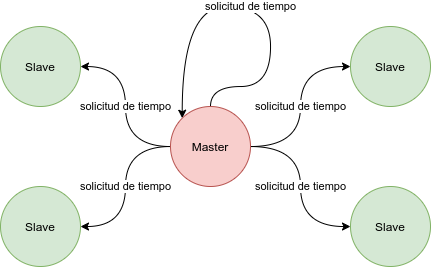
\includegraphics[width=10cm]{1}
  \caption{Solicitud de tiempo para cada Slave y el mismo Master}\label{fig:1}
\end{figure}

Después de la sincronización, cada proceso imprime su reloj lógico para
verificar el resultado de la sincronización.

El Slave maestro calcula la diferencia de tiempo promedio entre todas las horas
de reloj recibidas y la hora de reloj proporcionada por el reloj del sistema
maestro. Esta diferencia de tiempo promedio se agrega a la hora actual en el
reloj del sistema principal y se transmite a través de la red.

\begin{figure}[H]
  \centering
  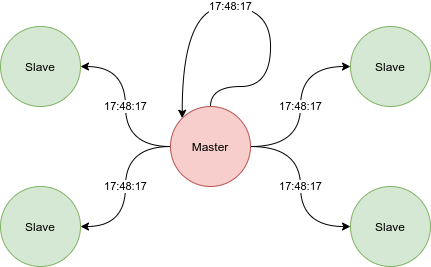
\includegraphics[width=10cm]{2}
  \caption{Sincronización del tiempo}\label{fig:2}
\end{figure}
\begin{listing}[H]
\inputminted[
  frame=lines,
  framesep=2mm,
  baselinestretch=1.2,
  bgcolor=LightGray,
  fontsize=\scriptsize,
  linenos,
  firstline=7,
  %lastline=49
  ]{python}{../berkeley/Workbench.py}
\caption{Implementación}
\label{lst:2}
\end{listing}

\begin{figure}[H]
  \centering
  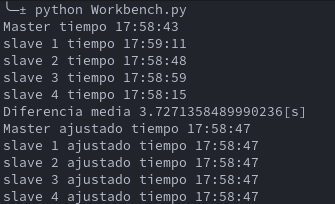
\includegraphics[width=8cm]{3}
  \caption{Ejecución de \mintinline{shell}{Workbrench.py}}\label{fig:3}
\end{figure}

\clearpage
\section{Algoritmo de Cristian}\label{sec:algor-de-cris}

El algoritmo de Cristian es un método para la sincronización de reloj que se
puede utilizar en muchos campos de la informática distributiva, los procesos
del cliente utilizan para sincronizar la hora con un servidor de
tiempo pero se utiliza principalmente en intranets de baja latencia.
El objetivo de este algoritmo es que es que todas las demás máquinas permanezcan sincronizadas con la \textit{maquina maestra}.
\begin{figure}[H]
  \centering
  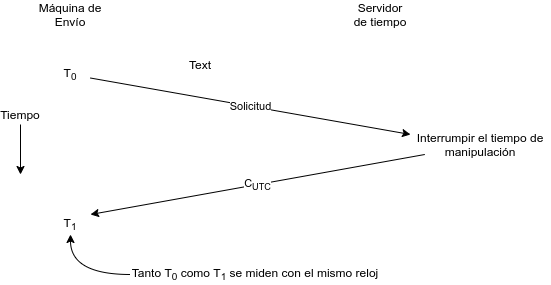
\includegraphics[width=10cm]{ac}
  \caption{Obtener la hora actual de un servidor.}\label{fig:4}
\end{figure}.

\begin{listing}[H]
\inputminted[
  frame=lines,
  framesep=2mm,
  baselinestretch=1.2,
  bgcolor=LightGray,
  fontsize=\scriptsize,
  linenos,
  firstline=7,
  %lastline=49
  ]{python}{../cristian/Workbench.py}
\caption{Workbench.py de algoritmo Cristian}
\label{lst:4}
\end{listing}

Inicializamos el maestro, hacemos uso de los sockets
\mintinline{shell}{tcp://localhost} junto con  puertos
$10000$, $10001$ y $10003$ para los Slaves y los registramos en el maestro
para después sincronizarlos.

\begin{listing}[H]
\inputminted[
  frame=lines,
  framesep=2mm,
  baselinestretch=1.2,
  bgcolor=LightGray,
  fontsize=\scriptsize,
  linenos,
  firstline=14,
  lastline=50
  ]{python}{../cristian/Server.py}
\caption{Server.py del algoritmo Cristian}
\label{lst:5}
\end{listing}
\clearpage

La clase \textsc{Cliente} se encarga de la implementación de los Slaves,
la cuál inicializa y, mediante una respuesta del Master (\textsc{Clase Server})
se sincroniza con ellos mediante el uso de la siguiente fórmula implementada
en el método \mintinline{shell}{obtener_tiempo} de la clase Server Código~\ref{lst:5}:
\begin{equation}
  \label{eq:1}
  \frac{T_{client}= T_{server}+(T_{1}-T_{o})}{2}
\end{equation}

Donde:

\begin{itemize}
  \item $T_{client}$ refiere a la hora del reloj sincronizado.
  \item $T_{server}$ refiere a la hora del reloj devuelta por el servidor.
  \item $T_{0}$ refiere  a la hora a la que el proceso del cliente envió la
        solicitud.
  \item $T_{1}$  a la hora a la que el proceso del cliente envió la solicitud,
\end{itemize}

\begin{listing}[H]
\inputminted[
  frame=lines,
  framesep=2mm,
  baselinestretch=1.2,
  bgcolor=LightGray,
  fontsize=\scriptsize,
  linenos,
  firstline=11,
  % lastline=50
  ]{python}{../cristian/Client.py}
\caption{Client.py del algoritmo Cristian}
\label{lst:6}
\end{listing}
\nocite{*}

\bibliographystyle{apalike}
\bibliography{ref}

\renewcommand\listoflistingscaption{Índice de códigos}
\newpage
\listoflistings\listoffigures
\end{document}
